\documentclass[journal,12pt,twocolumn]{IEEEtran}
\usepackage{setspace}
\usepackage{gensymb}
\singlespacing
\usepackage[cmex10]{amsmath}
\usepackage{amsthm}
\usepackage{mathrsfs}
\usepackage{txfonts}
\usepackage{stfloats}
\usepackage{steinmetz}
\usepackage{bm}
\usepackage{cite}
\usepackage{cases}
\usepackage{subfig}
\usepackage{longtable}
\usepackage{multirow}
\usepackage{enumitem}
\usepackage{mathtools}
\usepackage{tikz}
\usepackage{circuitikz}
\usepackage{verbatim}
\usepackage{tfrupee}
\usepackage[breaklinks=true]{hyperref}
\usepackage{tkz-euclide} % loads  TikZ and tkz-base
\usepackage{listings}
\usepackage{color}                                            %%
\usepackage{array}                                            %%
\usepackage{longtable}                                        %%
\usepackage{calc}                                             %%
    \usepackage{multirow}                                         %%
    \usepackage{hhline}                                           %%
    \usepackage{ifthen}                                           %%
  %optionally (for landscape tables embedded in another document): %%
    \usepackage{lscape}     
\usepackage{multicol}
\usepackage{chngcntr}
\lstset{frame=single,breaklines=true,columns=fullflexible}
\begin{document}
\def\putbox#1#2#3{\makebox[0in][l]{\makebox[#1][l]{}\raisebox{\baselineskip}[0in][0in]{\raisebox{#2}[0in][0in]{#3}}}}
     \def\rightbox#1{\makebox[0in][r]{#1}}
     \def\centbox#1{\makebox[0in]{#1}}
     \def\topbox#1{\raisebox{-\baselineskip}[0in][0in]{#1}}
     \def\midbox#1{\raisebox{-0.5\baselineskip}[0in][0in]{#1}}
\vspace{3cm}

\title{
ASSIGNMENT 2 - EE5600
	}
\author{ RS Girish - EE20RESCH14005$^{*}$% <-this % stops a space
	}	

\maketitle
\newpage
\tableofcontents
\bigskip
\renewcommand{\thefigure}{\theenumi}
\renewcommand{\thetable}{\theenumi}

\begin{abstract}
This paper contains solution to problem no 17 of 1.1 examples section.
Links to Python codes are available below.  
\end{abstract}
Download python codes using 
\begin{lstlisting}
https://github.com/rsgirishkumar/Assignment2/codes/
\end{lstlisting}
\section{Problem}
Consider the experiment of tossing a coin. If the coin shows head, toss it again but if it shows tail, then throw a die. Find the conditional probability of the event that "the die shows a number greater than 4" given that "there is at least one tail".\\
\section{Solution}
Let
\begin{center}
event A = tossing a coin,\\
event B = throwing a dice\\
\end{center}
for which\\
\begin{center}
sample size of A = 2
\begin{align*}
\Rightarrow S1={(heads,tails).}
\end{align*}
sample size of B = 6
\begin{align*}
\Rightarrow S2=(1,2,3,4,5,6).
\end{align*}
\end{center}
P(A)=P(tails)
\begin{align}
\Rightarrow P(A)=\frac{1}{2}
\end{align}
P(B)=P(dice showing number greater than 4)\\
\begin{align}
\Rightarrow P(B)=\frac{2}{6} \Rightarrow (5,6)
\end{align}
From Conditinal probability formula,
\begin{equation}
P(B/A)=P(A\cap B)/P(A)
\end{equation}
Since both are independent events,
\begin{equation}
P(A\cap B)=P(A)P(B)\\
\Rightarrow P(B/A)=P(B)
\end{equation}
Therefore
\begin{center}
P(dice throwing number greater than 4\\
given a tail when coin is tossed)
\begin{align*}
\Rightarrow P(B/A) = \frac {1}{3}
\end{align*}
\end{center}
The above is true for one toss but for n tosses\\
it will be a binomial distribution as below\\
\begin{equation}
 P(A=k)= { }^{n}C_{k}*p^{k}*q^{n-k} 
\end{equation}
indicating \\
p = probability of tails in individual event\\
q = probability of heads in individual event\\
n = number of trails of event\\ and\\
k = number of success i.e favourable outcomes of tails\\
For n=500, assuming equi-probable outcomes and only 1 success.\\
Theorotically,
\begin{align*}
P(A)=\frac{1}{2^{500}}\approx 0\\
\end{align*}
\\Using Binomial distribution,
\begin{equation}
P(A=1)= { }^{500}C_{1}*(0.5)^{1}*(0.5)^{500-1}
\end{equation}
\begin{align*}
\Rightarrow P(A=1) = 500 * 0.5^{500}\\
\Rightarrow P(A=1) \approx 0
\end{align*}
\\The PDF is of no relevance as P(A) = 0 will be more and it can be depicted as below.
\begin{figure}
	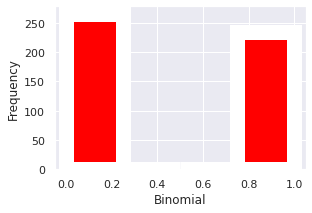
\includegraphics[width=\linewidth]{Binomial_1_success.png}
  \caption{Binomial Distriution of 500 tosses with 1 tail success.}
  \label{fig:Fig1}
\end{figure}
\\If only 1 success is available then
\begin{align*} 
P(B/(A=1))=P(B)
\Rightarrow =\frac{1}{3}
\end{align*}\\
Here given condition is "atleast one tail".Then k varies from 1 to 500 but not 0.Theorotically,\\
\begin{align*}
P(A)=1-\frac{1}{2^{500}}\approx 1
\end{align*}
\\Using Binomial distribution,
\begin{equation}
P(A > 0)=1-( { }^{500}C_{499}*(0.5)^{1}*(0.5)^{499})
\end{equation}
\begin{align*}
\Rightarrow P(A > 0) = 1-(500 * 0.5^{500})\\
\Rightarrow P(A > 0) \approx 1
\end{align*}
The PDF can be depicted as below\\
\\
\\
\begin{figure}
	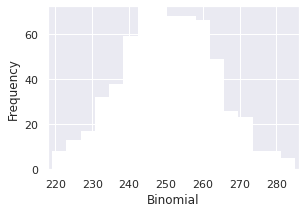
\includegraphics[width=\linewidth]{Binomial_500_success.png}
  \caption{Binomial Distriution of 500 tosses with many success.}
  \label{fig:Fig2}
\end{figure}
\\
\\
\\
\\
\\
\\
\\
\\
\\
\\
\\
\\When such success of tails are available as outcomes, the success of dice showing number greater than 4 also increases. This also follows a binomial distribution with total number of trials are number of successful outcomes i.e tails as outcome of coin tossing.Also, the event B is independent of event A.\\
\\Using Binomial distribution,
\begin{equation}
P(B>0)=( { }^{499}C_{k}*(\frac{1}{3})^{k}*(\frac{2}{3})^{499-k})
\end{equation}\\
\\
\\
\\
\\
\\
The PDF is given by
\begin{figure}
	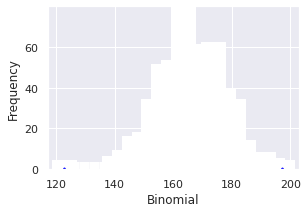
\includegraphics[width=\linewidth]{Numr_4_499_success.png}
  \caption{Binomial Distriution of Dice with many success i.e number greater than 4.}
  \label{fig:Fig3}
\end{figure}
\end{document}  